\chapter{Results}
\label{ch:results}

\section{Evaluation Metrics}
For model performance evaluation, we employ the standard measures of \textbf{precision}, \textbf{recall}, and \textbf{F1-score} from sequence labeling tasks. These are calculated at the token level such that each token prediction is compared against its respective ground truth label. A prediction is considered correct only if both the BIO tag and the corresponding field label (e.g., \texttt{B-TITLE}, \texttt{I-YEAR}) match the reference string annotated.

The metrics are computed with the \texttt{classification\_report} function of the \texttt{sklearn.metrics} module, which provides a per-class breakdown, together with macro- and weighted averages across all labels:
\begin{compactitem}
\item \textbf{Precision} is the proportion of predicted tokens for a label that were accurate.
\item \textbf{Recall} is the proportion of actual tokens correctly predicted.
\item \textbf{F1-score} is the mean of precision and recall, offering a balance of performance.
\end{compactitem}
Because of class frequency imbalance (for example, \texttt{O} tokens and \texttt{I-TITLE} are far more common than \texttt{B-ISSN} or \texttt{I-ISSUE}), we present \textbf{macro averages} (which are treating all labels equally) and \textbf{weighted averages} (which treats class frequency), because due to given class frequency imbalance we want to emphasize both overall model robustness and infrequent field type performance.
For example, in the CRF model, token-wise weighted F1-score was 0.91 with particularly high performance for often occurring fields \texttt{B-AUTHOR}, \texttt{I-TITLE}, and \texttt{B-PAGE}. More underrepresented labels \texttt{I-ISSUE} and \texttt{I-ISBN} achieved modestly lower recall as might be expected relative to their frequency within the corpus.


\section{Model Comparison}
\subsection{CRF Configurations}
During the first phase of experimentation, we experimented with a baseline CRF model with input features having solely \textbf{Byte-Pair Embeddings (BPEmb)}. It was trained on a dataset of 1 million labeled reference strings and served as the baseline to study the performance of semantic subword embeddings in isolation for citation parsing.

To examine if the mere encoded token-level cues would improve performance, we enriched the feature set by adding \textbf{hand-engineered features} derived from the AnyStyle parser~\cite{anystyle}. These included affixes, punctuation type, character case, semantic class, and position. The new model, again trained on 1 million samples, utilized a concatenation of BPEmb and these additional features.
The result was substantial improvement across all field tags with the exception of the most common ones. Precisely, F1-scores on structurally ambiguous or poorly documented fields (e.g., \texttt{B-ISSUE}, \texttt{B-DOI}, \texttt{I-CONTAINER-TITLE}) increased, which suggests that hand-engineered features helped the model detect syntactic boundaries and semantic roles harder to acquire from embeddings.

Encouraged by this progress, we ramped up CRF training to leverage \textbf{5 million} annotated examples and preserve both handcrafted features and BPEmb. Increased training size brought additional improvements, particularly in label consistency and low-frequency tag recall.
This line of models — from embeddings-only, to hybrid features, to large-scale training — illustrates how both feature sparsity and training size lead to better structured prediction performance on citation parsing tasks.
\begin{table}[h]
    \centering
    \begin{tabular}{|l|c|c|c|}
    \hline
    \textbf{Model} & \textbf{Training Size} & \textbf{Features Used} & \textbf{F1-score (Weighted Avg)} \\
    \hline
    CRF & 1 million & BPEmb only & 0.87 \\
    CRF & 1 million & BPEmb + Handcrafted & 0.90 \\
    CRF & 5 million & BPEmb + Handcrafted & 0.91 \\
    \hline
    \end{tabular}
    \caption[CRF Model Comparison (Features and Sizes)]{Comparison of CRF models with different features and dataset sizes using weighted F1-score.}
    \label{tab:crf_comparison}
\end{table}

As shown in Table~\ref{tab:crf_comparison}, we observe a consistent improvement in F1-score as we increase the feature richness and training data size. Adding handcrafted features to the BPEmb baseline improves the model's ability to capture structural cues in citation strings. Further increasing the training data to 5 million references yields additional gains, highlighting the importance of both quality and quantity in feature-based CRF models.


\subsection{BiLSTM + CRF}
To further improve performance over traditional CRF models, we implemented a \textbf{BiLSTM + CRF architecture} in PyTorch. This approach enables the model to capture contextual information in both forward and backward directions, making it especially suitable for structured sequence tasks like reference string segmentation. The model receives two types of input: dense contextual embeddings from Byte-Pair Encoding (BPEmb), and optionally, a projection of handcrafted features inspired by the AnyStyle parser. These features are embedded, projected to match the dimensionality of the BiLSTM output, and fused viaconcatinating them before being passed to the CRF decoding layer.

Two variants of the model were trained using \textbf{5 million reference strings}: one using only BPEmb, and the other using BPEmb with additional handcrafted features. Both models were evaluated on the same test set using token-level precision, recall, and F1-score. The results are summarized in Table~\ref{tab:bilstm_comparison}.
\begin{table}[h]
    \centering
    \begin{tabular}{|c|c|c|}
    \hline
    \textbf{Model} & \textbf{Features Used} & \textbf{F1-score (Weighted Avg)} \\
    \hline
    BiLSTM + CRF & BPEmb only & 0.86 \\
    BiLSTM + CRF & BPEmb + Handcrafted & 0.87 \\
    \hline
    \end{tabular}
    \caption[BiLSTM+CRF Feature Set Comparison]{Comparison of BiLSTM + CRF models trained on 5 million samples using different feature sets.}
    \label{tab:bilstm_comparison}
\end{table}

As shown in Table~\ref{tab:bilstm_comparison}, incorporating handcrafted features alongside BPEmb yielded a modest but measurable improvement in overall token-level F1-score. While both models benefited from the expressive power of bidirectional LSTMs, the inclusion of explicit structural cues contributed to more accurate field segmentation, especially in edge cases such as nested fields and punctuation-separated boundaries.

\subsection{BERT-based CRF Model}
To explore the effect of more advanced embeddings, we trained a CRF model using token-level embeddings generated by a modern \texttt{BERT-style encoder\\decoder}. Specifically, two different transformer-based architectures were evaluated:
\begin{compactitem}
\item \textbf{Linq-Embed-Mistral:} A recent multilingual model ranked highly on the Hugging Face embedding leaderboard for retrieval and semantic similarity tasks.
\item \textbf{DistilBERT Multilingual Cased:} A distilled and efficient version of BERT, offering faster inference with a modest trade-off in performance.
\end{compactitem}

Both models were used without additional handcrafted features or LSTM layers. The goal of these experiments was to determine whether high-quality contextual embeddings alone could match or surpass hybrid models that explicitly combine contextual and structural information.

The CRF models were trained on 5 million annotated reference strings using the BIO tagging scheme and evaluated using token-level precision, recall, and F1-score.
The results, summarized below, show that both BERT-based CRF models achieve competitive performance, with Linq-Embed-Mistral slightly outperforming DistilBERT in weighted F1-score. In particular, the Linq-Embed-Mistral model demonstrated superior performance on complex multi-token fields such as I-TITLE and I-AUTHOR, while DistilBERT achieved robust overall generalization with lower computational overhead. These findings suggest that leveraging strong pre-trained multilingual BERT based embeddings can effectively substitute for manual feature engineering when trained at scale.

\begin{table}[h] 
    \centering 
    \begin{tabular}{|l|c|} 
        \hline 
        \textbf{Model} & \textbf{F1-score (Weighted Avg)} \\ 
        \hline 
        CRF (Linq-Embed-Mistral) & 0.93 \\ CRF (DistilBERT Multilingual) & 0.92 \\ 
        \hline 
    \end{tabular} 
    \caption[BERT-based CRF Token-level Performance]{Token-level weighted F1-score performance of the CRF models using different BERT-style embeddings.} 
    \label{tab:bert_crf_comparison} 
\end{table}


\subsection{Final Comparison of Best Model Variants}
\label{subsec:final_comparison}
After analyzing each architecture independently, we summarize the performance of the best-performing configuration from each category in Table~\ref{tab:final_model_comparison}. The results clearly demonstrate the benefit of rich contextual embeddings provided by transformer-based models. The BERT + CRF configuration achieved the highest overall F1-score, followed by the traditional CRF using both BPEmb and handcrafted features. Interestingly, the BiLSTM + CRF model underperformed despite its ability to model sequential context, likely due to the difficulty of learning both token context and structure from scratch. This comparison highlights that pre-trained embeddings can substantially reduce the reliance on handcrafted features and outperform more complex neural architectures when applied effectively.
\begin{table}[h]
    \centering
    \begin{tabular}{|c|c|c|}
    \hline
    \textbf{Model} & \textbf{Features Used} & \textbf{F1-score (Weighted Avg)} \\
    \hline
    CRF            & BPEmb + Handcrafted     & 0.91 \\
    BiLSTM + CRF   & BPEmb + Handcrafted     & 0.87 \\
    BERT + CRF     & Linq-Embed-Mistral only & 0.93 \\
    \hline
    \end{tabular}
    \caption{Final comparison between the best-performing models from each architecture family.}
    \label{tab:final_model_comparison}
\end{table}

\begin{figure}[H]
    \centering
    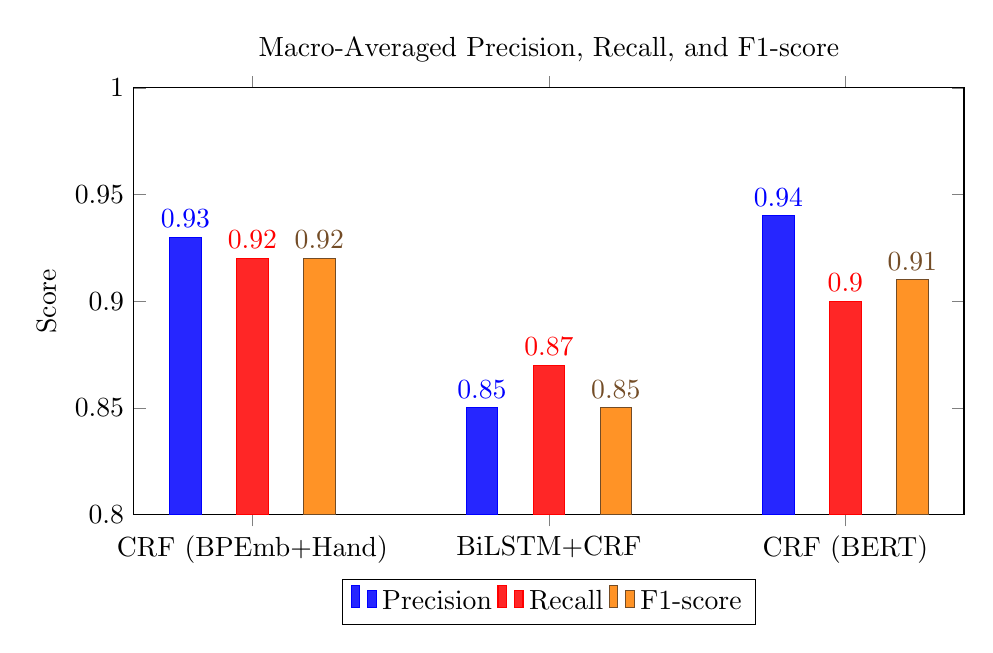
\begin{tikzpicture}  
    % Bar chart data
    \begin{axis}[
        ybar,
        bar width=.40cm,
        width=\textwidth,
        height=7cm,
        enlarge x limits=0.2,
        ylabel={Score},
        ymin=0.80, ymax=1.0,
        symbolic x coords={CRF (BPEmb+Hand), BiLSTM+CRF, CRF (BERT)},
        xtick=data,
        nodes near coords,
        nodes near coords align={vertical},
        legend style={at={(0.5,-0.15)}, anchor=north, legend columns=-1},
        xlabel={Model},
        title={Macro-Averaged Precision, Recall, and F1-score},
    ]
    \addplot+[style={fill=blue!85}, bar shift=-0.85cm] coordinates {
        (CRF (BPEmb+Hand),0.93) 
        (BiLSTM+CRF,0.85) 
        (CRF (BERT),0.94)
    };
    \addplot+[style={fill=red!85}, bar shift=0cm] coordinates {
        (CRF (BPEmb+Hand),0.92) 
        (BiLSTM+CRF,0.87) 
        (CRF (BERT),0.90)
    };
    \addplot+[style={fill=orange!85}, bar shift=0.85cm] coordinates {
        (CRF (BPEmb+Hand),0.92) 
        (BiLSTM+CRF,0.85) 
        (CRF (BERT),0.91)
    };

    \legend{Precision, Recall, F1-score}
    \end{axis}
\end{tikzpicture}
    \caption{Macro-level comparison of Precision, Recall, and F1-score across best-performing models.}
    \label{fig:model_comparison_chart}
\end{figure}

\subsection{Analysis of Results}
Based on the evaluation of the best-performing configurations across the CRF, BiLSTM + CRF, and BERT + CRF models, several insights can be drawn at both the macro and field-specific levels:
\begin{itemize}
\item \textbf{Model-Level Observations:}
\begin{compactitem}
\item \textbf{BERT + CRF}: achieved the highest overall weighted F1-score (0.93), along with the best precision (0.92) and recall (0.94). This confirms the effectiveness of transformer-based contextual embeddings, especially when used without additional handcrafted features.
\item \textbf{CRF (BPEmb + Handcrafted)}: performed surprisingly well with a weighted F1-score of 0.91, showcasing the strength of explicit token-level features when deep contextual embeddings are not available. Its performance was competitive with neural models across many fields.
\item \textbf{BiLSTM + CRF}, while offering contextual modeling through LSTM, slightly underperformed (F1-score: 0.87). This may be attributed to challenges in optimizing both the sequential context and structural features in a unified neural pipeline.
\end{compactitem}
\item \textbf{Field-Specific Insights:}
\begin{compactitem}
\item \textbf{Author Fields} (\texttt{B-AUTHOR}, \texttt{I-AUTHOR}): All models performed well on author detection, especially the BERT + CRF model, which reached F1-scores of 0.88 and 0.93 respectively. BiLSTM + CRF showed slightly lower precision on \texttt{B-AUTHOR}, indicating some sensitivity to name boundaries.
\item \textbf{Title Fields} (\texttt{B-TITLE}, \texttt{I-TITLE}): These fields consistently benefited from contextual embeddings. BERT + CRF achieved the best performance (\texttt{I-TITLE}: 0.94 F1), capturing long spans more effectively. The BiLSTM model also did well on \texttt{I-TITLE} due to its sequential memory, but struggled slightly with B-TITLE.
\item \textbf{URL Fields} (\texttt{B-URL}, \texttt{I-URL}): All models performed exceptionally on URLs, with F1-scores above 0.95. These fields are often easier to capture due to distinctive formatting (e.g., \texttt{http}, \texttt{www}, slashes), making them reliably detectable even by simpler models.
\item \textbf{DOI} and \textbf{PAGE}: Both BERT and CRF-based models achieved high performance on \texttt{B-DOI}, \texttt{B-PAGE}, and \texttt{I-PAGE}. These tokens also follow consistent patterns (numbers, slashes, etc.), allowing even non-contextual CRFs to generalize well.
\item \textbf{Container Title} (\texttt{I-CONTAINER-TITLE}): BiLSTM + CRF struggled here, achieving only 0.58 F1, while \textbf{CRF} and \textbf{BERT} models performed significantly better (0.87 and 0.85 respectively). This indicates that handcrafted features or pre-trained embeddings provide better signals for longer semantic chunks like journal names.
\item \textbf{Publisher} (\texttt{B-PUBLISHER}, \texttt{I-PUBLISHER}): The \texttt{I-PUBLISHER} tag was consistently well-handled across models (F1 near 0.90), but B-PUBLISHER showed more variability, reflecting challenges in distinguishing the beginning of organization names, especially when punctuation or unusual casing is involved.
\end{compactitem}
\end{itemize}

\subsection{Comparison with External Systems}
To place the performance of the new models in context, we compare their performance with previous work on bibliographic reference parsing. Despite potentially different conditions for datasets as well as evaluation policies, comparison provides an intuition of the relative position of the described methods.

\subsubsection{Evaluation Against a Large Language Model (GPT-4o)}
Recent advances in large language models (LLMs) have enabled strong performance on many natural language understanding tasks, even without explicit task-specific fine-tuning.
To explore how a general-purpose LLM would perform on bibliographic reference parsing, we used GPT-4o to label a sample of 100 reference strings.
The comparison offers insights into the strengths and limitations of applying a state-of-the-art LLM to a specialized sequence labeling task, without model retraining or task-specific adaptation.

Despite not having any task-specific tuning, GPT-4o did well on zero-shot general fields like \texttt{TITLE}, \texttt{PUBLISHER}, and \texttt{URL} with F1-scores greater than 0.90. Its performance was highly variable, however, on structured fields like \texttt{VOLUME}, \texttt{ISSUE}, \texttt{DOI}, and \texttt{ISBN}, where critical formatting details must be captured precisely. Our specialized models, however, like CRF with BPE and Handcrafted Features, BiLSTM+CRF, and CRF with BERT embeddings consistently outperformed GPT-4o across structured metadata fields. Overall, GPT-4o achieved a weighted F1-score of 0.89, while our best-performing models surpassed 0.91-0.93, confirming the value of task-specialized models for highly structured sequence labeling tasks like reference parsing.
\begin{figure}[H]
    \centering
    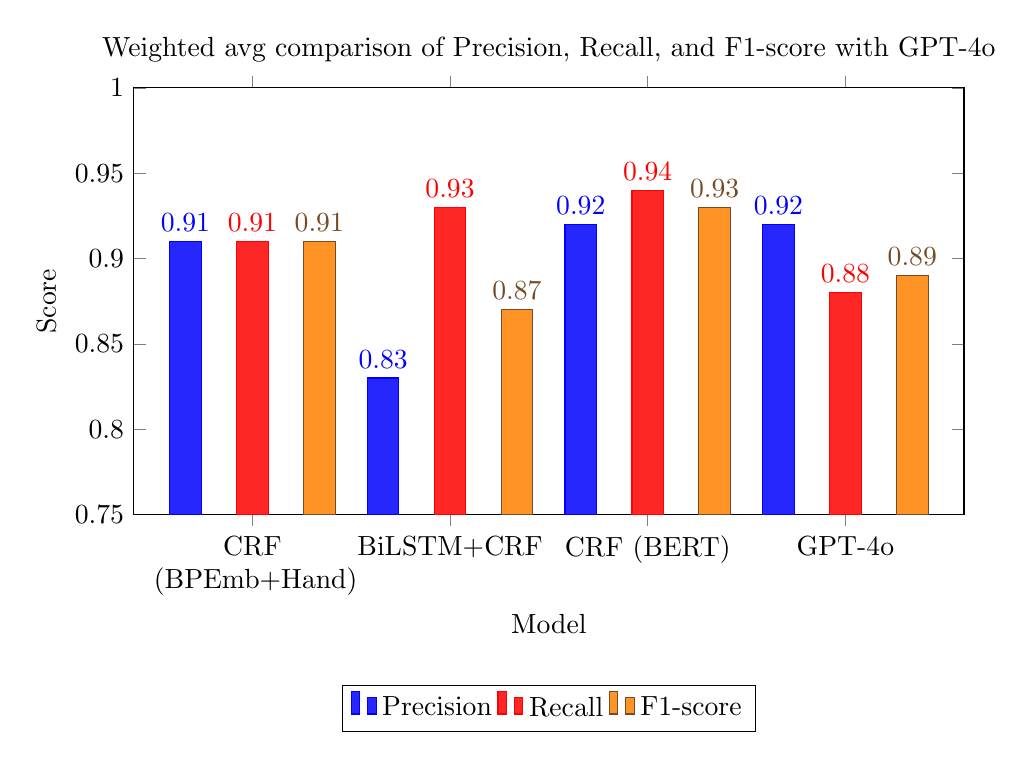
\begin{tikzpicture}
    \begin{axis}[
        ybar,
        bar width=0.40cm,
        width=\textwidth,
        height=7cm,
        enlarge x limits=0.2,
        ylabel={Score},
        ymin=0.75, ymax=1.0,
        symbolic x coords={CRF (BPEmb+Hand), BiLSTM+CRF, CRF (BERT), GPT-4o},
        xtick=data,
        xticklabel style={text width=2.5cm, align=center},
        nodes near coords,
        nodes near coords align={vertical},
        legend style={at={(0.5,-0.40)}, anchor=north, legend columns=-1},
        xlabel={Model},
        title={Weighted avg comparison of Precision, Recall, and F1-score with GPT-4o},
    ]
    
    \addplot+[style={fill=blue!85}, bar shift=-0.85cm] coordinates {
        (CRF (BPEmb+Hand),0.91) 
        (BiLSTM+CRF,0.83) 
        (CRF (BERT),0.92)
        (GPT-4o,0.92)
    };
    
    \addplot+[style={fill=red!85}, bar shift=0cm] coordinates {
        (CRF (BPEmb+Hand),0.91) 
        (BiLSTM+CRF,0.93) 
        (CRF (BERT),0.94)
        (GPT-4o,0.88)
    };
    
    \addplot+[style={fill=orange!85}, bar shift=0.85cm] coordinates {
        (CRF (BPEmb+Hand),0.91) 
        (BiLSTM+CRF,0.87) 
        (CRF (BERT),0.93)
        (GPT-4o,0.89)
    };
    
    \legend{Precision, Recall, F1-score}
    \end{axis}
\end{tikzpicture}
    \caption[Comparison of Best Models and GPT-4o]{Weighted-averaged Precision, Recall, and F1-score for the best performing models and GPT-4o.}
    \label{fig:comparison_gpt4o}
\end{figure}

\subsubsection{Comparison with External Published Work}
To put our models' performance into better perspective, we compare them to numbers published in independent studies. In particular, we compare our models' performance to the study by Cuéllar Hidalgo et al.~\cite{ArchComapre}, who have conducted an extensive evaluation of bibliographic reference parsing models. While their work shares some methodological similarity, the following key differences should be noted: their models were trained on much larger corpus (the full GIANT corpus), used no handcrafted features, and were evaluated on the CORA corpus — an independent test set from that employed in our experiments. Despite these differences, the comparison is worthwhile in so far as it gives insight into the relative design and performance of both approaches.

In their work, the BiLSTM+CRF model had a reported weighted F1-score of 0.96 while tested on the CORA dataset~\cite{ArchComapre} compared to both CRF-only and Transformer+CRF models. On our experiments, our top-performing BiLSTM+CRF model, which was trained using BPEmb embeddings and handcrafted features, achieved a weighted F1-score of 0.87 on our in-house large-scale test set. While our score is actually lower, note that our training set was much smaller (5 million references versus almost 200  million), and that hand-designed features were employed to augment performance instead of using learned embeddings exclusively.
Besides, while their evaluation used a standard dataset (CORA), our dataset more accurately sampled diverse and realistic styles of citations, with noisy and partial samples. This means our models retained good generalization behavior under more challenging situations.
\begin{figure}[H]
    \centering
    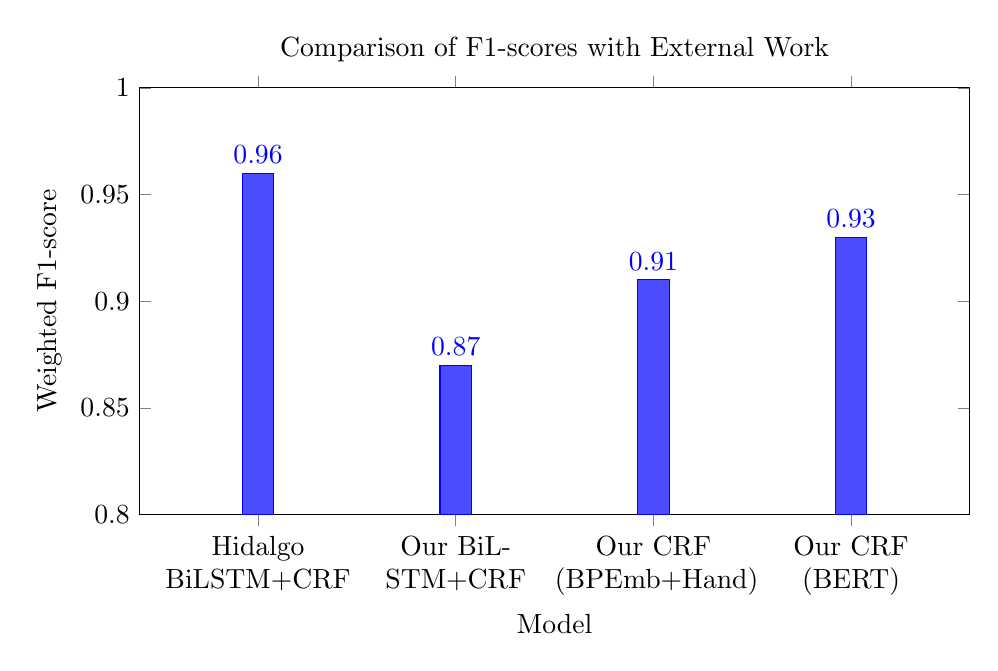
\begin{tikzpicture}
    \begin{axis}[
        ybar,
        bar width=.4cm,
        width=\textwidth,
        height=7cm,
        enlarge x limits=0.2,
        ylabel={Weighted F1-score},
        ymin=0.80, ymax=1.0,
        symbolic x coords={Hidalgo BiLSTM+CRF, Our BiLSTM+CRF, Our CRF (BPEmb+Hand), Our CRF (BERT)},
        xtick=data,
        xticklabel style={text width=2.5cm, align=center},
        nodes near coords,
        nodes near coords align={vertical},
        xlabel={Model},
        title={Comparison of F1-scores with External Work}
    ]
    \addplot+[style={fill=blue!70}] coordinates {
        (Hidalgo BiLSTM+CRF,0.96)
        (Our BiLSTM+CRF,0.87)
        (Our CRF (BPEmb+Hand),0.91)
        (Our CRF (BERT),0.93)
    };
    \end{axis}
\end{tikzpicture}
    \caption[Comparison of Weighted F1-Scores with External Published Work]{Comparison of weighted F1-scores between our models and the BiLSTM+CRF model from\cite{ArchComapre}.}
    \label{fig:external_comparison}
\end{figure}


